\let\textcircled=\pgftextcircled
\chapter{Positionnement du problème et Etat de l'art}
\label{chap:etat_de_lart}

\initial{C}\textit{e chapitre fait le tour des différents travaux qui proposent des solutions au problème d'estimation du WSS.}

\minitoc

\newpage    
\section{Enoncé du problème}
Comme mentionné à l'introduction, la mémoire est la ressource critique en terme de consolidation de VMs. Pour pallier ce problème, la solution la plus communément utilisée consiste à gérer la mémoire de la même façon que le processeur, i.e. d'effectuer une allocation de mémoire à la demande. 

\subsection{Allocation de mémoire à la demande}
Soit une VM dont la mémoire réservée a une capacité $\textit{m}_\textit{r}$ (représentant le \acs{SLA} \footnote{En français entente du niveau de service, c'est un document qui définit la qualité de service attendue et le niveau de service que souhaite obtenir un client de son fournisseur.}, \acl{SLA}, que le fournisseur ou l'hébergeur doit respecter), mais dont la mémoire activement utilisée est $\textit{m}_\textit{u}$ ($\textit{m}_\textit{u}$\leq $\textit{m}_\textit{r}$), l'approche d'allocation à la demande n'allouera à la VM qu'une quantité $\textit{m}_\textit{u}$ de mémoire (au lieu de $\textit{m}_\textit{r}$ comme avec une allocation statique) : $\textit{m}_\textit{u}$ est appelée \ac{WSS} de la VM \cite{article9}. Cette approche nécessite d'implémenter une boucle qui fonctionne comme suit :
\begin{itemize}
    \item L'activité de chaque VM est collectée périodiquement et sert d'\textit{input} à l'algorithme d'estimation du WSS
    \item Une fois l'estimation faite (notée $\textit{wss}_\textit{est}$), la mémoire allouée à la VM est ajustée à l'estimation faite $\textit{wss}_\textit{est}$
\end{itemize}
Ceci fait naître à deux principales interrogations : 
\begin{itemize}[label=\ding{42}, font=\large \color{darkorange}]
    \item \textbf{\large{\textcolor{darkorange}{(Q1)}}} Comment observer la VM et collecter les informations sur son activité sachant que celle-ci est une \textbf{«boîte noire»} pour l'hébergeur ?\\
    \item \textbf{\large{\textcolor{darkorange}{(Q2)}}} Une fois qu'on a répondu à (Q1), comment estimer le WSS de la VM à partir des données collectées ? \\
\end{itemize}
\par\noindent

\subsubsection{Répondre à Q1 : Comment collecter les informations sur l'activité mémoire de la VM ?}
Répondre à (Q1) soulève deux défis :
\begin{itemize}
    \item Le premier est relatif à la méthode à utiliser pour la collecte des données liées à l'activité mémoire de la VM. Une telle méthode peut être soit \textbf{active} soit \textbf{\textit{passive}}. Dans le premier cas, la méthode aura pour conséquence de modifier le cours d'exécution de la VM, ce qui n'est pas le cas pour une méthode passive.\\
    Une méthode active peut impacter sur les performances de la machine virtuelle. Par exemple, une façon triviale de traquer tous les accès mémoire est d'invalider (les marquer comme étant \textit{non présentes}) toutes les pages du \textit{shadow page table} (sous-section \ref{subsubsection:shadow_paging}) de la VM. Ainsi tous les accès subséquents produiront des défauts de page qui seront capturés par l'hyperviseur. Cette méthode peut en effet être catastrophique pour les performances de la VM à cause des coûts imputés par un défaut de page.
    
    \item Le deuxième défi se rapporte au niveau d'implémentation de la méthode utilisée. En effet, une telle méthode peut être implémentée à trois endroits : soit exclusivement dans l'hyperviseur (ou dans le dom0), soit exclusivement à l'intérieurde la VM, soit réparti à travers les deux. Dans les deux derniers cas, la méthode est dite \textbf{\textit{intrusive}} car la nature \textit{boîte noire de la VM} sera altérée. Dans cette circonstance, l'implémentation de la méthode nécessiterait l'accord du client.
\end{itemize}

\subsubsection{Répondre à Q2 : Comment estimer le WSS à partir des données collectées ?}
Concernant (Q2), les principaux défis à relever sont la \textbf{précision} de l'estimation et le coût lié à l'algorithme utilisé. En effet, étant donné qu'après estimation faite du WSS la mémoire allouée à la VM est réajustée, une estimation erronée pourrait soit impacter sur les performances de la machine, soit causer un gaspillage encore plus conséquent des ressources.

\subsection{Les métriques de l'estimation du WSS}
Les questions soulevées précédemment mettent l'accent sur les métriques à prendre en compte lorsqu'on définit un algorithme d'estimation pour le WSS :
\begin{itemize}[label=\ding{42}, font=\large]
    \item \textbf{Intrusive.} Une bonne méthode d'estimation ne devrait pas être intrusive, i.e. nécessiter la modification de la VM.
    \item \textbf{Active.} Une méthode active altére le flow d'exécution de la machine, ce qui n'est pas acceptable pour le client.
    \item \textbf{Précise.} L'estimation faite doit être précise pour éviter un réajustement erroné de la mémoire allouée à la VM.
    \item \textbf{Surcharge de la VM.} Une bonne méthode d'estimation ne doit pas engendrer des dégradations de performance de la VM. Ceci peut être la conséquence directe d'une méthode intrusive ou active.
    \item \textbf{Surcharge de l'hyperviseur.} Une surcharge importante peut saturer l'hyperviseur ou le dom0, ce qui pourrait conduire à des dégradations de performance des VMs.
\end{itemize}

\section{Les techniques existantes}
Dans cette section nous abordons les principales techniques proposées par des chercheurs. Pour chacune d'elles :
\begin{itemize}
    \item Nous présentons d'abord une brève description en montrant comment la technique répond aux questions Q1 \& Q2
    \item Ensuite nous expliquons sommairement la méthode d'implémentation dans XEN (qui est le système de virtualisation que nous utilisons)
    \item Et enfin nous présentons les forces et faiblesses de la solution
\end{itemize}  

\subsection{Self-ballooning}

\subsubsection{Description}
Le self-balloonig \cite{online6} repose essentiellement sur la VM, particulièrement sur son \acs{OS}.  
\par{\textbf{Réponse à Q1.}} Cette technique considère que le \acs{WSS} de la VM est donné par les statistiques du noyau, à l'occurrence le \textit{Committed\_As}\cite{online7, online8} \footnote{Quantité de mémoire, en kilooctets, nécessaire à la VM pour exécuter sa charge de travail. Elle représente la valeur du scénario le plus défavorable, incluant les défauts de page.} (\textit{cat /proc/mem/info}). Donc c'est l'OS lui même qui observe la VM et gère les appels d'allocation mémoire (\textit{malloc, etc.}), et calcule la mémoire totale allouée à tous les processus.
\par{\textbf{Réponse à Q2.}} L'OS décrémente le \textit{Committed\_As} chaque fois que des pages mémoire allouées sont libérées. Par exmple, considérons le processus qui exécute le programme C à la figure \ref{fig:exempl_prog_c} : après l'exécution de la ligne 2, la valeur du \textit{Committed\_As} est incrémenté de 2GB, même si uniquement 1octet est effectivement utilisé.

\begin{figure}[htp]
    \centering
    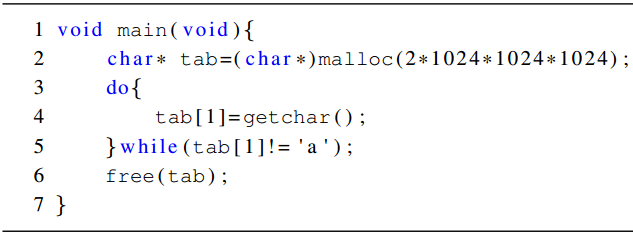
\includegraphics[scale=.65]{chapters/2/fig2/prog_c}
    \caption{Augmentation de la valeur du \textit{Committed\_As} avec l'instruction \textit{malloc} même si ne correspondant pas à la valeur de la mêmoire physique utilisée}
    \label{fig:exempl_prog_c}
\end{figure}

\noindent En somme, le \textit{Committed\_As} correspond au nombre total de pages mémoire virtuelles allouées par un processus, même si elles ne correspondent pas forcément à des pages physiques en mémoire centrale.

\subsubsection{Méthode d'implémentation}
Aucun effort d'implémentation n'est requis pour cette solution car c'est la technique utilisée par défaut dans XEN. En effet, XEN comme la plupart des hyperviseurs aujourd'hui, implémentent le \textit{memory ballooning}\cite{article9, article10}, une technique de gestion mémoire qui permet à l'hyperviseur de réclamer de la mémoire aux VMs et de la réallouer à d'autres. Dans cette technique, l'hyperviseur équipe chaque VM d'un \textit{balloon driver} qui peut être \textit{gonflé} ou \textit{dégonflé} dans le but d'augmenter ou de diminuer la mémoire allouée à la VM. Ainsi, en fonction de la valeur du \textit{Committed\_As}, l'hyperviseur va dynamiquement envoyer des instructions au \textit{balloon driver} de la VM qui va réajuster la mémoire de cette dernière.

\subsubsection{Caractéristiques et limites}
Comme présenté plus haut, cette méthode repose entièrement sur la VM. En outre, c'est le \textit{ballon driver} situé dans la VM qui se charge d'augmenter ou diminuer le cache de la machine, ce qui rend la solution très \textbf{intrusive}.\\
D'autre part, l'heuristique utilisée pour l'estimation du WSS, à savoir la valeur du \textit{Committed\_As}, n'est pas précise car elle ne prend pas en compte la mémoire cache. De ce fait, la mémoire estimée est la plupart du temps plus grande que celle activement utilisée par la VM, ce qui peut conduire à un gaspillage encore plus considérable des ressources.

\subsection{Zballoond}

\subsubsection{Description}
Zballoond \cite{zballoond} repose sur l'observation suivante : lorsque la taille de la mémoire allouée à la VM est supérieure à son WSS, le nombre de \textit{swap} est presque nul.
\par{\textbf{Réponse à Q1.}} L'idée basique derrière Zballoond est de diminuer graduellement la mémoire de la VM jusqu'à le nombre de \textit{swaps} commence à augmenter (devenir différent de zéro).

\par{\textbf{Réponse à Q2.}} Avec ce procédé, le WSS de la VM est donc considéré comme la plus petite taille mémoire qui maintient le nombre de \textit{swaps} à zéro.

\subsubsection{Méthode d'implémentation}
\textit{Zballoond} est implémenté à l'intérieur de la VM comme un module du noyau. L'algorithme d'implémentation boucle entre les étapes suivantes : 
\begin{enumerate}[label=\textbf{(\roman*)}]
    \item La mémoire de la VM est initialisée à sa valeur du \textit{Committed\_As}
    \item A chaque période (1 seconde par exemple), la mémoire est décrémentée par pourcentage du \textit{Committed\_As} (par exemple 5\%)
    \item Dès que la valeur du \textit{Committed\_As} change, \textit{Zballoond} considère que le WSS de la VM a également changé, et l'algorithme retourne à l'étape 1
\end{enumerate}

\subsubsection{Caractéristiques et limites}
Comme la méthode précédente, \textit{Zballoond} est entièrement implémentée dans l'OS de la VM ce qui la rend totalement \textbf{intrusive}.\\ 
De plus, c'est une technique très \textbf{active} en ce sens qu'elle force l'OS de la VM à réclamer des pages mémoire (à chaque période de l'étape de l'algorithme). Ainsi, les coûts imputés par cette méthode dépendent de la période d'observation et de la pression exercée sur la VM (quantité de mémoire réclamée).

\subsection{VMware}

\subsubsection{Description}
\textit{VMware} \cite{article10} est une amélioration de la technique naïve d'allocation à la demande. Au lieu d'invalider toutes les pages, la technique s'appuie sur une approche d'échantillonage Soit $\textit{m}_\textit{act}$ la taille actuelle de la mémoire de la VM.

\par{\textbf{Réponse à Q1.}} L'hyperviseur choisit périodiquement et aléatoirement $n$ pages dans la mémoire de la VM et les rend invalides (en les marquant \textit{non présentes} par exemple). Ainsi les prochains accès à ces pages généreront des exceptions qui seront capturées par l'hyperviseur.

\par{\textbf{Réponse à Q2.}} Une fois ces exceptions générées, l'hyperviseur compte le nombre $f$ de pages, parmi les pages précédemment sélectionnées dans l'échantillon, qui ont été sujettes à des défauts de page (pages marquées non présentes auxquelles la VM a tenté d'accéder). De cette façon, le WSS de la VM est estimé par la formule $ \frac{f}{n}* \textit{m}_\textit{act} $.

\subsubsection{Méthode d'implémentation}
Cette technique peut être implémentée de deux manières dépendemment de la façon dont les pages sont invalidées : soit en effaçant \footnote{Mettre le bit correspondant à 0} le bit de présence soit en effaçant le bit \textit{accessed}.\\
Entre le moment où les pages sont invalidées et celui où l'estimation du WSS est faite, l'hyperviseur va compter soit :
\begin{itemize}
    \item Le nombre de défauts de pages survenus, dans le cas où le bit de présence a été mis à 0.
    \item Le nombre de pages auxquelles la VM a accédées (parmi les pages de l'échantillon), dans le cas où le bit \textit{accessed} a été mis à 0. Dans ce second cas de figure, l'hyperviseur n'a pas à capturer une exception car le bit \textit{accessed} est automatiquement mis à 1 par le matériel lorsqu'un processus accède à une page.
\end{itemize}

\subsubsection{Caractéristiques et limites} 
Cette technique est \textbf{non intrusive} car entièrement implémentée dans l'hyperviseur/dom0. Toutefois, elle présente deux inconvénients majeurs : 
\begin{itemize}
    \item Le fait d'invalider les pages mémoire de la VM modifie son cours d'exécution, ce qui peut provoquer des dégradations de performances en fonction de la méthode d'implémentation : dans le cas où l'implémentation se fait en effaçant le bit de présence des pages, les dégradations sont plus importantes (dues aux coûts de résolution d'un défaut de page). Toutefois, dans le cas c'est le bit \textit{accessed} qui est mis à 0, la précision de l'estimation peut être biaisée si l'hyperviseur/dom0 exécute d'autres programmes susceptibles de remettre ce bit à 0.
    \item \textit{VMware} est incapable d'estimer un WSS supérieur à la mémoire actuellement allouée à la VM. En effet, dans le meilleur des cas l'algorithme déterminera que toutes les pages de la machine ont été accédées et estimera ainsi le WSS à la taille actuelle de la mémoire.
\end{itemize}

\subsection{Geiger}

\subsubsection{Description}
\textit{Geiger} \cite{geiger} répond aux questions 1\&2 tel qu'il suit.

\par{\textbf{Réponse à Q1.}} Pour observer l'activité mémoire de la VM, la technique consiste à surveiller les évictions et mise à jour éventuelles du cache de la VM vers la partition de swap.

\par{\textbf{Réponse à Q2.}} \textit{Geiger} repose sur une technique appelée \textit{buffer fantôme} \cite{ghost_buffer}. Ce dernier est un buffer imaginaire qui étend la mémoire physique de la VM ($\textit{m}_\textit{act}$). La taille de ce buffer représente la quantité de mémoire supplémentaire qui doit permettre d'éviter à la VM d'effectuer des \textit{swap out} de pages mémoire. Ainsi l'estimation du WSS de la VM se fait à travers la formule : $ WSS = \textit{m}_\textit{act} + \textit{m}_\textit{fant}$ si $\textit{m}_\textit{fant} > 0 $.

\subsubsection{Méthode d'implémentation}
Le challenge pour implémenter cette technique est de pouvoir isoler le traffic du swap des autres requêtes d'entrée/sortie, dans le but de forcer la VM à utiliser un autre pilote comme partition de swap. Ce pilote est spécialement configuré pour l'implémentation de la technique, de la façon suivante : lorsqu'une page est éjectée de la mémoire de la VM, une référence à cette page est ajoutée à une file dans le pilote situé dans le dom0. Plus tard, lorsqu'une page est lue depuis la partition de swap, \textit{Geiger} retire la référence à cette page de la file et calcule la distance $D$ de la page à la tête de file. C'est cette distance $D$ qui représente le nombre de pages mémoire supplémentaires, nécessaire à l'OS de la VM pour éviter des \textit{swap out}.

\subsubsection{Caractéristiques et limites}
Tout comme \textit{VMware}, \textit{Geiger} est totalement transparente du point de vue de la VM, et ne nécessite donc pas de permission de la part du client. Toutefois ce caractère non intrusif de la technique pose un sérieux problème. En effet, \textit{Geiger} n'est capable d'estimer le WSS que si la taille de la \textit{mémoire fantôme} strictement positive, i.e. si la VM est dans un état de \textit{swap}. \textit{Geiger} devient donc inefficace si le WSS de la machine est inférieure à la mémoire qui lui est actuellement allouée.

\subsection{Hypervisor Exclusive Cache}

\subsubsection{Description}
\textit{Exclusive Cache} \cite{exclusive_cache} est assez similaire de \textit{Geiger} en ce sens qu'il repose également sur la notion de buffer fantôme pour estimer le WSS.\\
Ici chaque VM détient une petite quantité de mémoire appelée mémoire directe, le reste étant gérée par l'hyperviseur sous forme de \textbf{cache exclusif}. C'est ce cache exclusif qui est considéré dans cette technique comme la mémoire fantôme (dans le cas de \textit{Geiger}). Ainsi, une fois que la VM consomme toute sa mémoire directe, elle swap ses pages non pas vers la partition de swap mais vers l'hyperviseur.

\subsubsection{Méthode d'implémentation}
Tout comme \textit{Geiger}, \textit{Exclusive Cache} est implémenté sous forme d'une extension disque. Mais ici à la place d'un pilote de disque externe comme avec \textit{Geiger}, le contenu des pages de la VM peut être sauvegardé dans un buffer situé dans le dom0, qui matérialisera le buffer fantôme.

\subsubsection{Caractéristiques et limites}
À l'opposé de \textit{Geiger}, cette technique est plus active dans la mesure où elle oblige la VM à être dans un état de swap, étant donné qu'il y a une partie de sa mémoire qui est conservée par l'hyperviseur.\\
Quoiqu'il en soit, les impacts de performance sont moindres car l'extension de disque est contournée et les pages mémoire de la VM sont enregistrées dans le dom0.

\subsection{Dynamic MPA ballooning}

\subsubsection{Description}
Le \textit{Dynamic MPA \footnote{Dynamic Memory Pressure Aware} ballooning} \cite{dmpa} étudie la gestion de la mémoire du point de vue de l'ensemble de la machine hôte.

\par{\textbf{Réponse à Q1.}} \textit{MPA ballooning} introduit un ensemble d'hypercalls à traver lesquels toutes les VMs reportent à l'hyperviseur le nombre de leurs pages mémoire. 
\par{\textbf{Réponse à Q1.}} Sur la base de ces informations, l'algorithme définit trois niveaux possibles de pression de la mémoire : 
\begin{itemize}
    \item Bas : le nombre de pages mémoire de toutes les VMs est inférieur à la mémoire physique totale de l'hôte.
    \item Moyen : le nombre de pages mémoire de toutes les VMs est égal à la mémoire physique totale de l'hôte.
    \item Elevé : le nombre de pages mémoire de toutes les VMs est supérieur à la mémoire physique totale de l'hôte.
\end{itemize}

\noindent En fonction de l'état de pression de la mémoire, l'OS adopte une politique de gestion différente : 
\begin{itemize}
    \item Dans le cas d'un niveau de pression bas, cette technique divise la mémoire disponible dans l'hyperviseur en ($nb_VMs + 2$) parts. Chaque part est assignée à une VM comme mémoire réservée et les deux autres sont maintenues par l'hyperviseur en cas de demande soudaine. Chaque part est vue comme le cache exclusif dans la méthode \textit{Hypervisor Exclusive Cache}.
    \item Dans le cas d'un niveau de pression moyen, l'hyperviseur réclame les pages inactives à toutes les VMs et les rééquilibre en ($nb_VMs + 1$) parts.
    \item Enfin dans le cas d'un niveau de pression élevé, la technique éjecte toutes les pages du cache et rééquilibre exclusivement les pages anonymes.
\end{itemize}

\subsubsection{Caractéristiques et limites}
\textit{Dynamic MPA} est très intusif étant donné qu'il nécessite des hypercalls supplémentaire de l'OS de la VM. C'est une technique qui n'est donc réellement effective que dans le cas d'un datacenter privé où le gestionnaire a un contrôle plus élevé sur les VMs. En outre, ces nouveaux hypercalls exportent des données précises et importantes sur la couche mémoire des VMs, ce qui accroît le risque d'attaques sur les machines.